\documentclass[12pt]{article}
\usepackage{graphicx}
\usepackage[margin=1.0in]{geometry}   % sets all margins to 1in, can be changed
\usepackage{moreverb}                 % for verbatimtabinput -- LaTeX environment
\usepackage{rotating}
\usepackage{url}     
\usepackage{hyperref}
\usepackage{multirow}
\usepackage{amssymb}                  % for many mathematical symbols
\usepackage[pdftex]{lscape}           % for landscaped tables
\usepackage{longtable}
\usepackage[dvipsnames]{xcolor}
\usepackage[spanish]{babel}
\usepackage[utf8]{inputenc}


\newtheorem{Def}{Definici\'on}[section]
\newtheorem{Ejem}{Ejemplo}[section]
\newtheorem{Teo}{Teorema}[section]
\newtheorem{Dem}{Demostraci\'on}[section]
\newtheorem{Note}{Nota}%[section]
\newtheorem{Sol}{Soluci\'on}[section]
\newtheorem{Prop}{Proposici\'on}[section]
\newtheorem{Coro}{Corolario}[section]



\title{Un primer estudio estad\'istico de la Certificaci\'on en la UACM}
\author{Carlos E. Martínez-Rodríguez\thanks{Departamento de Estadística, Universidad Autónoma de la Ciudad de México (UACM). Correo electrónico: carlos.martinez@uacm.edu.mx}}
\date{27 de noviembre de 2022}

\begin{document}
\maketitle
\tableofcontents

\section{Introducci\'on y antecedentes}


\subsection{Artículo 1: Machine Learning in Enzyme Engineering}
Título: \href{https://pubs.acs.org/doi/full/10.1021/acscatal.9b04321}{Machine Learning in Enzyme Engineering, Stanislav Mazurenko, Zbynek Prokop, and Jiri Damborsky} \cite{Mazurenko}

\begin{itemize}
\item Enzyme engineering is the process of customizing new biocatalysts with improved properties by altering their constituting sequences of amino acids.

\item Multiple ML algorithms have already been applied to enzyme engineering. Some notable examples include random forests used to predict protein solubility \cite{15}, support vector machines \cite{16,17} and decision trees \cite{18} to predict enzyme stability changes upon mutations, K-nearest-neighbor classifiers to predict enzyme function\cite{19} and mechanisms,\cite{20} and various scoring and clustering algorithms for rapid functional sequence annotation \cite{21,22}. The main attractiveness of ML in enzyme engineering stems from its generalizability: once it is trained on the known input, called a training set, an ML algorithm can potentially make predictions about new variants almost instantly.

\item The aim of this Perspective is, therefore, to highlight recent advances in data collection and algorithm implementation for ML in enzyme engineering. 

\end{itemize}

\subsection{The essence of Machine Learning}

La esencia de la mayoría de los algoritmos de Machine Learning (ML) es encontrar patrones en los datos disponibles, datos que consisten en varios descriptores o características, por ejemplo secuencias de encimas, sus estructuras secundarias y terciarias, substiruciones, etc.  El nímero de características usualmente varían de decenas a miles lo que convierte el problema en uno de alta dimensión. 

\begin{figure}{ht!}
\centering
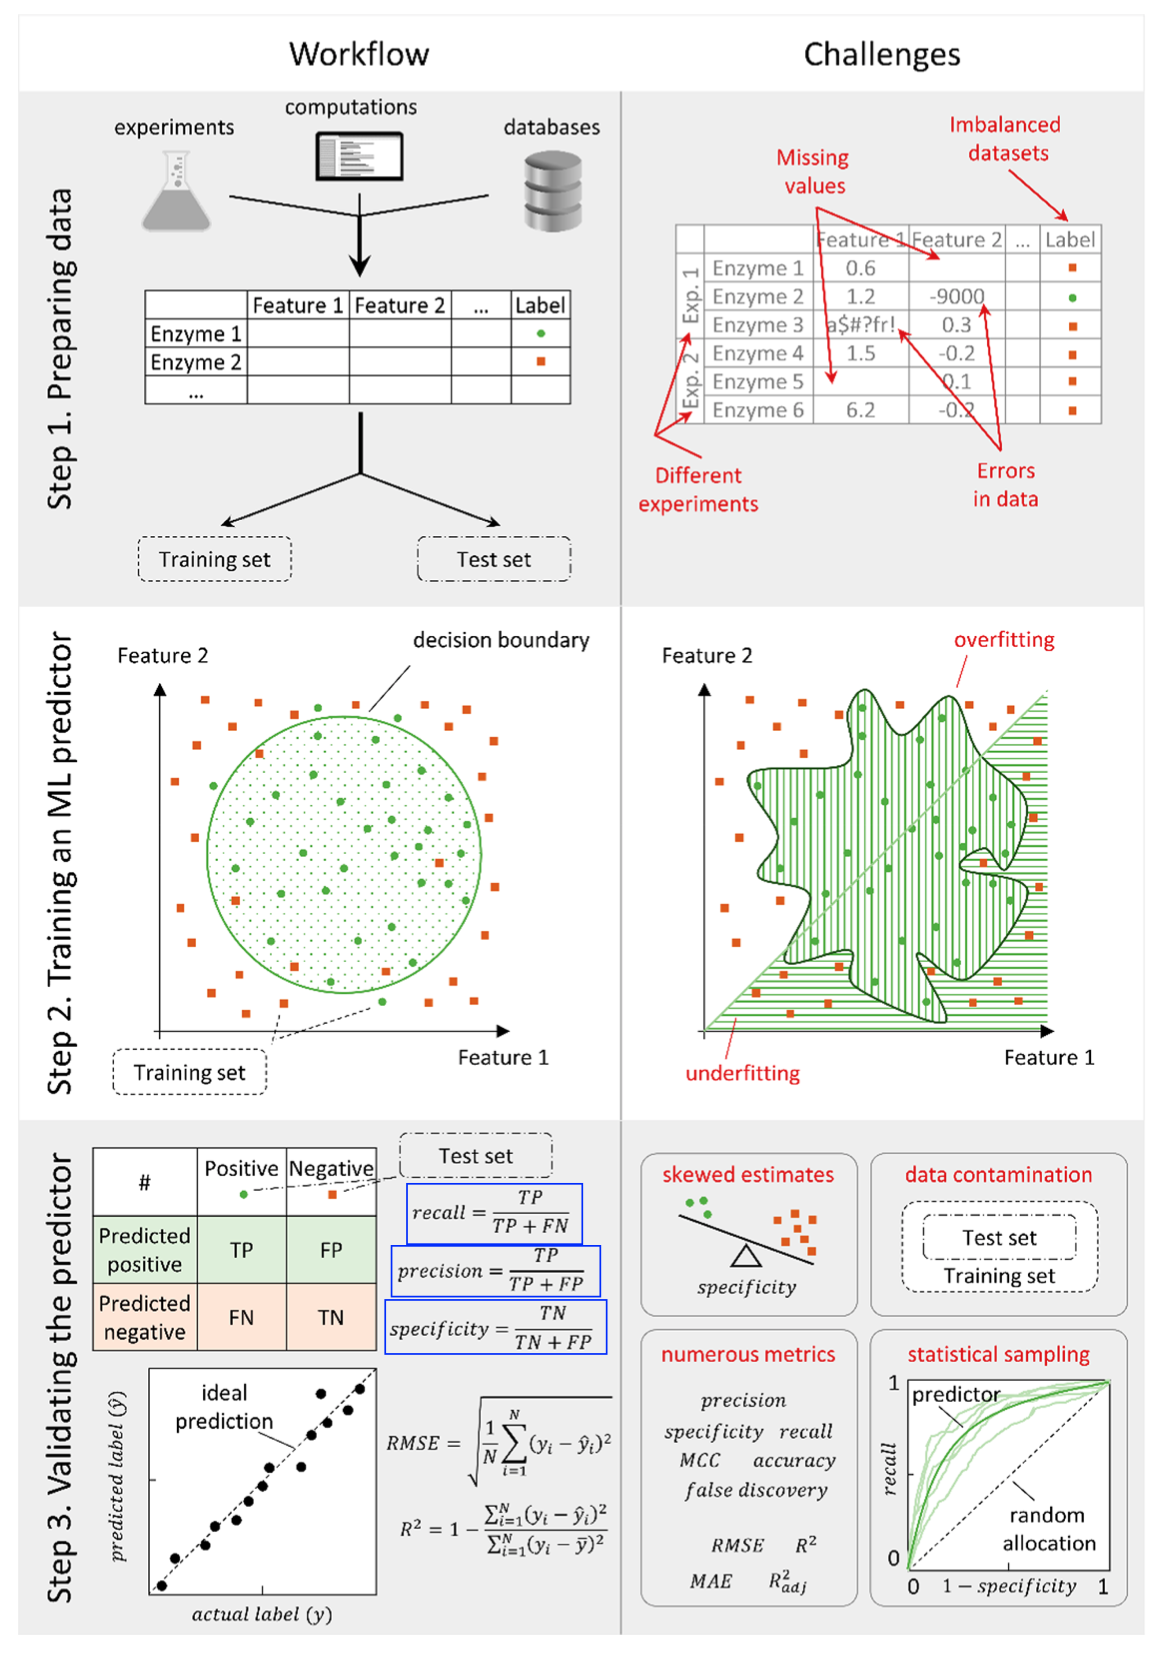
\includegraphics[scale=0.45]{Figura2.png}
\caption{Schematic workflow of constructing an ML predictor and associated challenges. }
\label{Figura2}
\end{figure}

Los principales tipos de Machine Learning son: Aprendizaje Supervisado y Aprendizaja No-Supervisado. En el aprensizaje no supervisado el objetivo es disminuir la alta dimensionalidad de los datos en uno de menor dimensión, o el de encontrar clústers en los datos.  En el aprendizaje supervisado varias propiedades objetivo tales como actividad o estabilidad de enzimas,  y el objetivo es diseñar un predictor que regrese etiquetas para datos no vistos considerando sus descriptores,  utilizando el conjunto de datos etiquetado como datos de entrenamiento.

\begin{Note}
Step 1: the data are usually turned into a table format and split into the training and test parts. Any errors, biases, or imbalances will be translated to the predictor’s performance and, hence, must be accounted for. Step 2: the predictor is trained on the training data set. For example, a decision boundary is derived that allows classifying future input based on whether data points are inside or outside the boundary. This is a balancing act between two extremes: explaining noise rather than fundamental dependencies (overfitting) or failure to account for complex dependencies in the data (underfitting). Step 3: the performance of the predictor is evaluated based on the test data set. For example, true and false positives and negatives and the associated measures are calculated or the root mean square error (RMSE) is calculated for continuous labels. The random nature of the initial data split as well as data imbalances might skew the evaluation, and numerous metrics used for evaluation vary in their robustness to different data skews. Even partial inclusion of the test set at any stage of ML predictor training is called data contamination and usually invalidates the final evaluation.

\end{Note}


La etapa que más tiempo consume es la de recolección de datos y su preparación para alimentar el algoritmo de ML, entonces los datos son introducidos en el subconjunto de entrenamiento, el resultado se utiliza para meujorar los parámetros del predictor de ML, mientras que el segundo se utiliza para la evaluación. 


\begin{Note}
\begin{itemize}

\item En problemas de clasificación con etiquetas binarias o etiquetas con una cantidad finita de opciones, la evaluación usualmente se realiza por medio de la matriz de confusión: el número de verdaderos/falsos positivos y negativos.

\begin{center}
\begin{tabular}{|c|c|c|}\hline
& Positivo & Negativo\\\hline
Predecido Positivo& TP & FP\\\hline
Predicido Negativo& FN & TN\\\hline
\end{tabular}
\end{center}

\item Para problemas de regresión con etiquetas de valores continuos usualmente se calcula la raíz del error cuadrático medio

\begin{equation}
RMSE=\sqrt{\frac{1}{N}\sum_{i=1}^{N}\left(y_{i}-\hat{y}\right)^2}
\end{equation}


\begin{equation}
R^2=1-\frac{\sum_{i=1}^{N}\left(y_{i}-\hat{y}\right)^2}{\sum_{i=1}^{N}\left(y_{i}-\overline{y}\right)^2}
\end{equation}

\end{itemize}

En cualquiera de los dos casos la evaluación final se lleva a cabo en el conjunto de prueba, el cuál es esencial dado que el último objetivo es obtener el predictor más general en los datos no utilizados para entrenar el algoritmo.
\end{Note}


\begin{Note}
Las siguientes métricas se utilizan para medir el rendimiento de un modelo en función de su capacidad para predecir correctamente las clases de un conjunto de datos. 

\begin{itemize}

\item \textbf{Recall (Recall o Sensibilidad):} Conocido como sensibilidad o tasa positiva real, mide la capacidad de un modelo para identificar correctamente todos los ejemplos positivos en un conjunto de datos. Se calcula como el número de verdaderos positivos dividido por la suma de verdaderos positivos y falsos negativos:

\begin{equation}
Recall = \frac{Verdaderos\ Positivos}{Verdaderos\ Positivos + Falsos\ Negativos}
\end{equation}

Un recall alto significa que el modelo es bueno para detectar los casos positivos, minimizando los falsos negativos. Es importante en situaciones donde los falsos negativos son costosos o críticos.


\item Precision (Precisión): La precisión mide la capacidad de un modelo para predecir correctamente los casos positivos entre todas las predicciones positivas que realiza. Se calcula como el número de verdaderos positivos dividido por la suma de verdaderos positivos y falsos positivos:

\begin{equation}
Precision = \frac{Verdaderos\ Positivos}{Verdaderos\ Positivos + Falsos\ Positivos}
\end{equation}

Una alta precisión significa que el modelo tiene una baja tasa de falsos positivos, es decir, que cuando predice una clase como positiva, es probable que sea correcta. La precisión es importante en situaciones en las que los falsos positivos son costosos o no deseados.

\item Specificity (Especificidad): La especificidad mide la capacidad de un modelo para predecir correctamente los casos negativos entre todas las predicciones negativas que realiza. También se conoce como tasa negativa real. Se calcula como el número de verdaderos negativos dividido por la suma de verdaderos negativos y falsos positivos:

\begin{equation}
Specificity=\frac{Verdaderos\ Negativos}{Verdaderos\ Negativos+Falsos\ Positivos}\end{equation}
Una alta especificidad indica que el modelo es bueno para identificar correctamente los casos negativos, minimizando los falsos positivos. Esto es importante en situaciones en las que los falsos positivos son costosos o problem\'aticos.
\end{itemize}
Estas métricas proporcionan una forma más completa de evaluar el rendimiento de un modelo de clasificación que simplemente mirar la precisión general. 
\end{Note}


En la ingeniería de proteínas, las similitudes en secuencias en ambos subconjuntos de datos deben ser tenidas en cuenta. Si alguna familia de proteínas está sobre representada en el conjunto de prueba, el predictor resultante puede resultar sesgado hacia la identificación de patrones válidos solamente para esta familia. Si algunas secuencias en el conjunto de prueba son muy cercanas al conjunto de entrenamiento, la evaluación final de desempeño dara resultados sobre optimistas. 

En el paso 2 de entrenamiento, es posible ajustar el predictor o seleccionar de entre varios predictores, usualmente por medio de validación $k-fold$. En este caso los datos de entrenamiento se subdividen en $K$ subconjuntos y el flujo de trabajo se repite $K$ veces, con cada uno de ellos utilizaods para la evaluación de los $K-1$ subconjuntos utilizados para entrenar. El reto principal en el paso 2 para cualquiern entrenamiento tipo ML supervisado es evitar el subajuste de los datos (sesgo alto) y el sobre ajuste (varianza grande). 

La \textbf{subestimación} ocurre cuando un predictor falla en encontrar patrones incluso en los datos de entrenamiento (cuando un modelo lineal simple se utiliza para explicar dependencia dependencias no lineales en los datos). El \textbf{sobreajuste} ocurre cuando el desempeño de un predictor disminuye notablemente en los datos de prueba en comparación con los datos de prueba, debido al aprendizaje de demasiado detalle y ruido, en lugar de identificar patrones generales. Tanto el subajuste como el sobreajuste pueden ser debido a la insuficiente calidad de los datos: ruido excesivo, características faltantes o irrelevantes, sesgo en los datos, o datos dispersos. También pueden ocurrir como consecuencia de una pobre aplicación del algoritmo: excesiva o insuficiente flexibilidad en la selección de los parámetros, protocolo de entrenamiento inapropiado, o contaminación de los datos de entrenamiento con el conjunto de datos de prueba.


\subsection{Bases de datos relevantes a Ingeniería de Enzima}


\subsubsection{The State of the Art in Data Accumulation}

Debido a que los algoritmos de ML se basan en los datos, la importancia de la calidad de los mismos utilizados para entrenamiento no puede ser subestimada.

Ejemplos de conjuntos de bases de datos, utilizadas en la ingeniería de enzimas, son secuencias de proteínas y estructuras de proteínas. La estabilidad y solubilidad de las proteínas son dos cualidades que han sido medidas por varias décadas y hasta la fecha. Tareas más desafiante es la anotar las propiedades catalíticas de las enzimas debido a la abundancia de tipos de reacciones, mecanismos, cofactores, amplios rangos de especificidades de sustratos, enancionselectividades y promiscuidades.


Las enzimas son catalizadores biológicos que facilitan una amplia variedad de reacciones químicas en los organismos vivos. Algunas razones por las cuales la anotación de sus propiedades catalíticas es complicada son:

\begin{itemize}
\item \textbf{Tipos de reacciones diversos:} Las enzimas pueden catalizar una amplia gama de reacciones químicas, incluyendo reacciones de oxidación-reducción, hidrólisis, condensación, isomerización y más. Cada tipo de reacción involucra mecanismos químicos y sustratos diferentes.

\item \textbf{Mecanismos:} Incluso dentro de un solo tipo de reacción, las enzimas pueden emplear múltiples mecanismos. Comprender el mecanismo específico utilizado por una enzima requiere un conocimiento detallado de la estructura de la enzima y de su sitio activo.

\item \textbf{Cofactores:} Muchas enzimas requieren cofactores, como iones metálicos o coenzimas, para catalizar reacciones de manera efectiva. Identificar los cofactores necesarios para cada enzima es esencial para la anotación.

\item \textbf{Condiciones de reacción:} La actividad enzimática puede depender en gran medida de las condiciones ambientales, incluyendo la temperatura, el pH y la fuerza iónica. La anotación de las condiciones óptimas para la actividad enzimática es crucial.

\item \textbf{Especificidades de sustratos:} Las enzimas pueden ser altamente específicas para ciertos sustratos, reconociéndolos con alta afinidad, mientras que otras son más promiscuas y pueden unirse a una variedad de sustratos. La caracterización de la especificidad de sustratos es compleja.

\item \textbf{Enantioselectividades:} Algunas enzimas pueden discriminar entre enantiómeros (isómeros de imagen especular) de una molécula, catalizando reacciones con alta selectividad por un enantiómero. La anotación de esta propiedad implica comprender la estereoquímica.

\item \textbf{Promiscuidades:} Las enzimas pueden exhibir actividades promiscuas, catalizando reacciones diferentes a su función principal. Detectar y caracterizar tales promiscuidades es complicado.
\end{itemize}

\subsubsection{Current Challenges Related to Databases}

Si la dependencia que se busca no se encuentra en los datos disponibles, no importa la cantidad de nuevos datos ayudarán a mejorar la calidad del predictor de ML. En el caso de la ingeniería de enzimas se espera que las funciones enzimáticas estén codificadas en las secuencias y así depender en las propiedades físico-químicas de los aminoácidos, de aquí que la cantidad y la calidad de los datos en las bases de datos sean de importancia para diseñar un predictor de ML.


La falta de estándares en los reportes resulta en pérdida de información o valores erróneos para algunos descriptores. A esto hay que agregar la falta de protocolos robustos en los análisis de datos, como por ejemplo aquellos utilizados para ajuste de curvas para determinar las temperaturas de fusión o constantes cinéticas. Otro factor es que los recientes avances vuelven obsoletos resultados previos. La curación manual ayuda mejorar la calidad de los datos, sin embargo no se encuentra excenta de errores de anotación de las funciones de las proteínas y errores de propagación a partir de resultados previamente refutados.

Este tipo de procedimientos, verificación manual, puede incluir la limpieza o formato de datos para que sean amigables con ML. Uno de los principios más populares es \textbf{FAIR}, por sus siglas en inglés, Findable, Accesible, Interoperables y Reutilizables, debería de facilitar a las computadoras para que de manera automática pueda encontrar y utilizar los datos. Para las enzimas la guía estándar para reportar datos de enzimas (STRENDA) debería de aumentar la calidad de los datos, especialmente en bases de datos (bdd) heterogéneas recopiladas de diversas fuentes.


El desarrollo de nuevos predictores de ML ha incrementado considerablemente la demanda de mejora de las bdd existentes, así como la generación de nuevas bdd uniformes y representativas de mayor calidad. 

Existen varias nuevas técnicas emergentes tales como

\begin{itemize}
\item[i ] Secuenciación de nueva generación.
\item[ii ] Clasificación de células activadas por fluorescencia.
\item[iii ]  Exploración mutacional profunda, y  
\item[iv ] Microfluidos

\end{itemize}

\subsubsection{Emerging Methods for High-Throughput Data
Collection}

Avances tecnológicos hacia la miniaturización, automatización y paralelización han generado tecnologías eficientes de nuevos métodos de investigación experimental con capacidades incomparables. Secuenciación de nueva generación (NGS) ha revolucionado la investigación genómica, habilitado el acceso a datos moleculares fundamentales y revelado firmas genómicas  y transcriptomicas \cite{47,48}.

La capacidad de secuencias en el rango de gigabases por ejecución del instrumento permite secuencias el genoma humano en su totalidad en tan sólo un día. 

Múltiples instrumentos comerciales de segunda generación disponibles ofrecen mayor capacidad y precisión. Métodos de tercera generación recientemente introducidos (lectura larga)  que emplean secuenciación en tiempo real de moléculas \cite{50} o secuenciación de nanoporos \cite{51} resuelve las limitaciones de lecturas cortas, como el sesgo de GC o mapear elementos repetitivos

Mientas el avance de la tecnología de secuenciación proporciona una gran cantidad de secuencias de datos, para la mayoría de estas entradas, las anotaciones estructurales y anotaciones funcionales aún están perdidas. 


Como siguiente paso, se está centrando en el desarrollo de nuevos métodos experimentales efectivos para recopilar información funcional y estructural. 

La clasificación de células activadas por fluorescencia (FACS) es una tecnología ampliamente disponible que permite el cribado de hasta 108 variantes de enzimas por día. La FACS requiere que los sustratos fluorogénicos estén atrapados dentro o en la superficie de la célula para vincular el genotipo y el fenotipo. Alternativamente, se utiliza la clasificación de enzimas encapsuladas junto con su ADN codificador y un sustrato fluorogénico en perlas de hidrogel.

Cuando se combinan con la secuenciación de próxima generación, los ensayos de alto rendimiento representan una estrategia poderosa para analizar de manera integral las relaciones entre secuencia y función en las enzimas \cite{52,55}. Este enfoque, llamado escaneo mutacional profundo (DMS por sus siglas en inglés), vincula el genotipo con el fenotipo sin necesidad de procesos laboriosos que involucren la purificación y caracterización de proteínas. Durante el proceso, se sintetiza una gran biblioteca de secuencias mutantes, seguida de la selección de fenotipos expresados. Luego, la secuenciación de la biblioteca antes y después de la selección cuantifica la aptitud de cada mutante. De esta manera, el DMS proporciona un método rápido y sencillo para inferir los determinantes de la secuencia de la estabilidad y la función de las proteínas\cite{52,56,57}. El DMS se ha utilizado como una estrategia experimental alternativa para la determinación de la estructura de las proteínas.


\subsection{MACHINE LEARNING APPLICATIONS TO ENZYME ENGINEERING}

\begin{itemize}

\item Despite being a relatively new field of study,  machine Learning for enzyme engineering has already been applied for several challenging predictions.  First consider predictors aimed at elucidating the structure function relationships crucial for enzymes on both sides:

\begin{itemize}
\item predicting the structure for a known sequence, and 

\item predicting the catalytic activity or substrate specificity for a known sequence-structure. 
\item solubility and stability, from the point of view of amino acid substitutions,

\end{itemize}

\item The protein structure prediction is one of the longest-standing challenges in biochemistry, as the number of resolved structures is dramatically lagging behind the number of known sequences.

\item Over 145000 structures have been released in the Protein Data Bank, but this is still nowhere near over 215 million publicly available protein sequences\cite{28}. 

\item Nevertheless, even despite a relatively small data set size in comparison to millions of data points usually available for this method, deep neural networks showed most the notable results in the latest biennial assessment of protein structure prediction methods, CASP13. 

\begin{Note}
The AlphaFold network was trained on the PDB entries to predict the distances between C-beta atoms of residues using multiple sequence alignments\cite{60} and received the highest score at the competition. Out of 124 targets, around two-thirds of AlphaFold predictions had a $GDT_TS$ score above 50, which is indicative of a topologically correct structure \cite{61}.
\end{Note}

\item Apart from predicting protein structures, predicting catalytic activities is another active field of research currently. 

\item Computational methods for the protein function prediction range from sequence-to structure-based and from gene-to genome- and interactome-based\cite{62}. 


\item Several initiatives similar to the CASP competition have already been proposed to address the functional annotation of enzymes, namely Enzyme Function Initiative (EFI), the Computational Bridges to Experiments initiative (COMBREX), and the Critical Assessment of Function Annotation community-driven experiment (CAFA). 


\item Successful attempts to apply ML to assign enzyme EC numbers using predicted 3D structures \cite{63} or exploiting sequence similarities \cite{64} have already been made. 

\item Recently, deep learning was also applied to predict EC numbers on the basis of a protein sequence using both sequence-length-dependent features, such as raw sequence one-hot encoding, and sequence-length-independent features, such as functional domain encoding \cite{65}.


\item The former type of features introduced non uniformity in feature dimensionality, and the authors presented a framework to perform simultaneously dimensionality uniformization,  feature selection, and  classification model training. 

\item The large data sets of enzyme structures and activities accumulated to date already allow using deep learning in the engineering of catalytic activity. 


\item A more precise functional prediction is possible by restricting ML training to a particular family of enzymes, which comes at the cost of much smaller data sets available for training. This problem may be tackled by applying high-throughput data collection methods mentioned before. The authors of the recently released GT-predict \cite{66} selected for their analysis the glycosyltransferase superfamily 1, a group of enzymes with highly diverse substrates. 


\begin{Note}
Data from the label-free mass spectroscopy-based assay of 91 substrates and 54 enzymes derived from the plant Arabidopsis thaliana were used for functional prediction. The authors trained sequence-based decision trees, systematically varying combinations of physicochemical  properties,  e.g. log P, molecular area, and number/type of nuclephilic groups, and structural information, e.g.  scaffold type and functional groups. The resulting predictor was successfully tested on four individually selected gene sequences as well as two complete families of enzymes from four different organisms, which highlights the tremendous potential of training ML predictors on the newly acquired data from high-throughput data collection methods. 
\end{Note}

\item In their recent paper \cite{35} Han and coauthors considered seven different binary and continuous ML algorithms: logistic regression, decision tree, support vector machines,  Naive Bayes,  conditional random forest,  XGBoost, and artificial neural networks. 

\item The authors attempted to use generative adversarial networks to synthesize more data. This is a pair of two neural networks competing against each other: one learns to generate artifficial examples and the other to distinguish them from real data. 

\item Another point of view on protein solubility prediction is studying the effects of individual mutations. The recent successes in the application of deep mutational scanning to collect the data on protein solubility changes upon mutations\cite{68} are likely to promote the development of more sophisticated ML-based protein solubility predictors in the nearest future. 

\item Predicting the effects of amino acid substitutions is not only limited to solubility: stability, substrate specificity, catalytic activity, and enantioselectivity can also be targeted if sufficient data are available.


\item Protein stability predictors are perhaps those with the most abundant data sets of this type available for ML training

\item The authors also presented a random forest classiffier trained using 1106 features from the following groups: experimental conditions, conservation and coevolution scores for mutated positions, amino acid substitutions and their physicochemical properties, neighborhood features for 11 positions before and after substitution sites, and thermodynamic sequence-based features extracted from ProtDCal \cite{69}. 


\item PON-tstab is a three-class predictor (stability increasing, decreasing, unchanged) and achieved the correct prediction ratio of around 0.5 versus the value 0.33 for a random predictor. This implies that, even with a data set of higher quality, predicting protein stability remains an extremely challenging task \cite{5}.

\item Another intriguing application of ML in protein engineering is to design smart combinatorial libraries for directed protein evolution\cite{70}. This has the potential to both reduce the experimental effort and improve the exploration of the sequence space by mutating multiple positions simultaneously. Moreover, it can approximate the empirical fitness landscape to suggest a refined set of variants for the next round of screening.

\item Wu et al\cite{71} used ML assisted directed evolution to engineer an enzyme for a new stereodivergent carbon-silicon bond formation. The authors selected the reaction of phenyldimethyl silane with ethyl 2-diazopropanoate catalyzed by a putative nitric oxide dioxygenase from Rhodothermus marinus. They tested a variety of ML algorithms such as linear and kernel models, shallow neural networks, and ensemble methods to improve the enzyme enantioselectivity.

\end{itemize}


 
\subsubsection{Current Challenges Related to ML-Aided}

\begin{itemize}

\item One of the main challenges in applications of ML to enzyme engineering stems from the intrinsic multidisciplinarity of the approach. Biochemists, molecular biologists, mathematicians, and computer scientists have to find a common language to clarify goals, carry out rigorous analysis and training, and avoid common pitfalls, wrongful usage of methods, and misinterpretations.

\item The No Free Lunch theorem \cite{85} claims that no single ML method is superior to others a priori \cite{86}; 


\item A thorough understanding of the data types to be used and problems to be solved is essential in the development of efficient predictors. The current shift toward new and more complex ML methods, namely aggregating several algorithms into hybrid meta-predictors, hyperparameter optimization with many training subcycles, feature learning, and the fusion of ML-based and classical bioinformatics tools in a single predictor, will further challenge the crosstalk between disciplines necessary for the development of efficient and robust predictors in enzyme engineering.

\item With the continuous growth of ML applications in enzyme engineering, the need for robust comparison of various predictors is of growing importance. This comparison is mainly obstructed by the lack of both standardized protocols for comparison and new data sets for testing. 

\item The lack of benchmark data sets, discrepancies in the performance measurements used, inaccurate or insufficient disclosure in publications, and the difficulty in finding reviewers with sufficiently broad expertise \cite{87} are among the most pressing issues. 

\item Researchers working on some applications with a long track record in bioinformatics, such as protein structure or function predictions, have already established several platforms that can be used for comparison of the ML predictors, i.e. CASP, CAFA, EFI, and COMBREX.

\item Other applications have yet to see similar initiatives as at least three key ingredients are necessary: 

\begin{itemize}
\item[i] a sufficiently large community of researchers working on development of such applications, 
\item[ii] a sufficient amount of new high-quality data being collected regularly, and 
\item[iii] a leader that will take on responsibility and invest time and effort into coordinating this activity. 
\end{itemize}

\item Few papers go beyond simple ROC analysis: e.g., resample cross-validation to estimate its statistical significance, explore the reasons for weak predictions, and analyze learning curves. Why does a particular predictor have a better performance? What features are critical for the performance of a predictor on a global scale? What ranges for feature values and what parts of the feature space are most critical for a particular data point to be classiffied correctly?
\end{itemize}

\subsection{Emerging Trends in ML-Based Methods for Enzyme Engineering}


\begin{itemize}
\item With the accumulation of more data by virtue of the emerging high-throughput experimental methods, the development of benchmark data sets and unified performance measurements is only a matter of time.

\item Recently, an intriguing algorithm based on semisupervised learning has been presented to allow benchmarking in five different prediction tasks related to protein engineering, including secondary structure, fluorescence landscape, and stability landscape predictions \cite{88}

\item As the data generation is streamlined, a data set from a single experiment is starting to have the size large enough for training ML algorithms to guide the design of future experiments, as was the case in the development of stereodivergent carbon silicon bond formation\cite{71} and the application of Gaussian processes to the directed evolution of cytochromes\cite{89}.

\item The increase in the available data will prompt more extensive use of deep neural networks. Sophisticated neural network architectures, such as recurrent or graph-based neural networks, simultaneous training of several types of predictors (multitasking), combining structurally different input data (multimodal design), ML-based modeling of data sets (generative models), and retraining predictors used in one area by new data from another area (transfer learning) have only recently been applied in genomics\cite{14}


\item Several attempts have recently been made to apply some of those advanced techniques to proteins: using generative models to create soluble and functional malate dehydrogenase variants\cite{90} or predict mutational effects with high correlation with those actually observed in 42 high-throughput deep mutational scanning experiments\cite{91}


\item More data will also allow improving the existing methods, i.e. learning the optimal architecture of a predictor from the data (hyperparameter optimization)\cite{92}, smart aggregation of several predictions from multiple methods\cite{93}, and introducing robust conffidence scores for predictions\cite{94}. In enzyme engineering, this new level of algorithmic complexity will further save time and resources wasted on validating misleading predictions but will also require more sophisticated computer architecture, e.g. an increased use of parallel computing and stochastic training methods, which have already become standard techniques for the acceleration of deep neural network training.



\item Another noticeable trend in ML is toward interpretable and explainable predictors\cite{95}. Apart from the global importance of features for ML predictors, feature importance scores calculated for each input example\cite{96,97} may help explain why a particular prediction was made for each input data point. 


\item Interpretable algorithms can aid in smart biocatalyst design. For instance, instead of simply screening all the possible mutations with an ML-based tool to improve a target property, researchers can make use of designing variants on the basis of the structure of a predictor using adaptive sampling\cite{98}. 



\item Such an approach favors predictors whose parameters can provide such guidance: e.g., linear predictors over more flexible yet harder to interpret artifficial neural networks (Figure 3). Linear predictors allow analytical design on the basis of the coefficients \cite{99} in contrast, sophisticated predictors are usually prone to pathological behavior, i.e. sudden misclassiffication after a slight and almost imperceptible perturbation of input\cite{100}.


\item Another promising approach is to use interpretable architectures of predictors already at the design stage, e.g. the visible neural networks\cite{101}. The design of such networks is guided by the knowledge of the underlying biological mechanism, e.g. the choice of layers and the connections between layers may mimic the hierarchical organization of transcriptional regulatory factors in the cell nucleus.


\end{itemize}










\section{Artículo 2: A general model to predict small molecule substrates of enzymes based on machine and deep learning}

\subsection{About the existence techniques}

\begin{Note}
\begin{itemize}
\item Las enzimas han evolucionado de manera eficiente para catalizar eficientemente una o más reacciones químicas incrementando las tasas de reacción hasta más de un millón. Además la mayoría de las enzimas son promiscuas, es decir, se catalizan más, fisiológicamente irrelevantes o reacciones inofensivas \cite{2.2, 2.4}

\item Un mapeo exhaustivo de las relaciones enzima-sustrato desempeña un papel crucial en la investigación farmacéutica y bioingeniería, por ejemplo, para la producción de medicamentos, productos químicos, alimentos y biocombustibles \cite{2.5, 2.6,2.7}.


\item La base de datos UniProt contiene entradas de más de 36 millones de enzimas diferentes, más del $99\%$ de ellas carecen de anotaciones de alta calidad de las reacciones catalizadas. Se están realizando esfuerzos para desarrollar métodos de alto rendicmiento para la determinación experimentarl de relaciones entre enzimas y sustratos, esfuerzos que se encuentran en su etapa inicial\cite{2.9,2.10,2.11}.


\item Se han realizado esfuerzos por desarrollar metodos de alto rendimiento para determinar las relaciones experimentales de las relaciones enzima-sustratos. El objetivo en este trabajo es desarrollar un modelo de Machine Learning (ML) con la capacidad de predecir las relaciones enzima-sustratos a traves de todas las proteínas, por tanto contar con una herramienta que ayude a focalizar esfuerzos experimentales en pares de moléculas de pequeñas enzimas parece ser biológicamente relevantes. 

\item Los principales retos son que la representación numérica de caeda enzima que máximamente informativa para la predicción rio abajo, para ser lo más ampliamente posible, estas representaciones deben basarse de manera única en la secuencia primaria de las enzimas sin información adicional. Otro reto es que las bases de datos públicas de enzimas, solamente enlista instancias positivas, es decir, moleculas con las cuales las enzimas despliegan actividades medibes \cite{2.13}. 

\end{itemize}
\end{Note}

\subsection{About the ML techniques}

\begin{Note}
\begin{itemize}
\item Para entrenar un modelo de predicción, es necesario idear una estrategia automatizada para obtener instancias adecuadas de enzimas y pequeñas moléculas que sean negativas y no se unan. Los enfoques de aprendizaje automático existentes para predecir pares enzima-sustrato fueron desarrollados específicamente para familias de enzimas pequeñas para las cuales existen conjuntos de datos de entrenamiento inusualmente completos \cite{2.13}-\cite{2.18}.

\item Mou et al.\cite{2.14} desarrollaron modelos para predecir los sustratos de las nitrilasas bacterianas, utilizando características de entrada basadas en las estructuras tridimensionales y sitios activos de las enzimas. Entrenaron varios modelos de aprendizaje automático basados en evidencia experimental para todas las posibles combinaciones de enzima y molécula pequeña dentro del alcance de predicción de los modelos (N = 240). 


\item Yang et al.\cite{2.15} predijeron el alcance de sustratos de las glicosiltransferasas de plantas entre un conjunto predefinido de moléculas pequeñas. Entrenaron un modelo basado en árboles de decisión con un conjunto de datos que cubría casi todas las posibles combinaciones de enzimas y moléculas pequeñas relevantes. 


\item Pertusi et al.\cite{2.13} entrenaron cuatro máquinas de vectores de soporte (SVM) diferentes, cada una para una enzima específica. Como características de entrada, sus modelos solo utilizan información sobre los sustratos (potenciales), así como no sustratos extraídos manualmente de la literatura; no se utilizó información explícita sobre las enzimas.


\item Roettig et al.\cite{2.16} y Chevrette et al.\cite{2.17} predijeron los alcances de sustratos de familias de enzimas pequeñas, entrenando modelos de aprendizaje automático con información estructural relacionada con los sitios activos de las enzimas. 


\item Visani et al.\cite{2.19} implementaron un modelo de aprendizaje automático general para predecir clases EC adecuadas para un sustrato dado. Para entrenar este modelo, se utilizaron todas las clases EC que no están asociadas con un sustrato específico como puntos de datos negativos, lo que resultó en una baja proporción promedio de positivos a negativos de 0.0032. Visani et al. no utilizaron información sobre las enzimas más allá de la clase EC como entrada del modelo, y por lo tanto, el modelo no puede distinguir entre diferentes enzimas asignadas a la misma clase EC.


\end{itemize}
\end{Note}

\subsection{About the approuch of existing models}

\begin{Note}

\begin{itemize}
\item Todos estos modelos no pueden aplicarse a enzimas individuales o intentan predecir sustratos solo para una enzima o familia de enzimas. 

\item Aquellos modelos que hacen predicciones para enzimas específicas se basan en datos de entrenamiento experimentales muy densos, es decir, resultados experimentales para todas o casi todas las posibles combinaciones de enzima-sustrato.

\item Para la gran mayoría de familias de enzimas, no está disponible un conjunto de datos de entrenamiento tan extenso. 

\item Hasta el momento, no ha habido intentos publicados de formular y entrenar un modelo general que pueda aplicarse para predecir sustratos para enzimas específicas en familias de enzimas ampliamente diferentes. 

\item Los modelos de aprendizaje profundo se han utilizado para predecir funciones de enzimas ya sea prediciendo su asignación a clases EC20–22, o prediciendo dominios funcionales dentro de la secuencia de proteínas\cite{2.23}

\item Predecir directamente sustratos específicos para enzimas representa un paso importante más allá de esos métodos previos y puede ayudar a predecir la función de la enzima de manera más específica y precisa.

\item Los enfoques de vanguardia en este dominio son basados en características, es decir, se utilizan representaciones numéricas de la proteína y la molécula del sustrato como entrada para modelos de aprendizaje automático\cite{2.25}-\cite{2.29}. 

\item Como descripciones numéricas de la molécula del sustrato, estos enfoques utilizan representaciones SMILES30, huellas digitales expertas\cite{2.31} o huellas digitales creadas con redes neuronales gráficas\cite{2.32,2.33}. 

\item Las proteínas suelen codificarse numéricamente mediante representaciones basadas en el aprendizaje profundo de las secuencias de aminoácidos\cite{2.34}-\cite{2.36}.

\end{itemize}

\end{Note}

\subsection{About the work in this article}

\begin{Note}
\begin{itemize}

\item In this work, we go beyond the current state-of-the-art by creating maximally informative protein representations, using a customized, task-specific version of the ESM-1b transformer model34. 

\item The model contains an extra 1280-dimensional token, which was trained end-to-end to store enzyme-related information salient to the downstream prediction task. 

\item This general approach was first introduced for natural language processing37, but has not yet been applied to protein feature prediction. 

\item We created negative training examples using data augmentation, by randomly sampling small molecules similar to the substrates in experimentally confirmed enzyme-substrate pairs.

\item we sampled all negative data points from a limited set of metabolites, the set of ~ 1400 substrates that occur among all experimentally confirmed enzyme-substrate pairs of our dataset. 

\item Thus, we do not sample from the space of all possible alternative reactants similar to the true substrates, but only consider small molecules likely to occur in at least some biological cells. 

\item While many enzymes are rather promiscuous2–4, it is likely that most of the potential secondary substrates are not contained in this restricted set for any given enzyme, and hence the chance of sampling false negative data points was likely small. 

\item We numerically represented all small molecules with task-specific fingerprints that we created with graph neural networks (GNNs)38–40. 

\item A gradient-boosted decision tree model was trained on the combined protein and small molecule representations for a high-quality dataset with ~18,000 very diverse, experimentally confirmed positive enzyme-substrate pairs (Fig. 1). 

\item The resulting Enzyme Substrate Prediction model-ESP-achieves high prediction accuracy for those ~1400 substrates that have been part of our training set and outperforms previously published enzyme family-specific prediction models.
\end{itemize}

\end{Note}

\subsection{About the obtained results}

\begin{Note}
\begin{itemize}


\item A data set with experimentally confirmed enzyme-substrate
pairs using the GO annotation database for UniProt IDs41  was created.

\item For training the machine learning models, they extracted 18,351 enzyme-substrate pairs with experimental evidence for binding, comprised of 12,156 unique enzymes and 1379 unique metabolites. 

\item Also extracted 274,030 enzyme-substrate pairs with phylogenetically inferred evidence, i.e., these enzymes are evolutionarily closely related to enzymes associated with the same reactions. These “guilt by association” assignments are much less reliable than direct experimental evidence, and we only used them during pre-training to create task-specific enzyme representations-numerical vectors aimed at capturing information relevant to the prediction task from the enzyme amino acid sequences. 

\item The validations demonstrate that using phylogenetically inferred functions for the construction of appropriate enzyme representations has a positive effect on the prediction of experimentally confirmed enzyme-substrate pairs.

\item There is no systematic information on negative enzyme-small molecule pairs, i.e., pairs where the molecule is not a substrate of the enzyme.

\item It was hypothesized that such negative data points could be created artificially through random sampling, which is a common strategy in classification tasks that lack negative training data \cite{2.42}.


\item Only were considered small molecules included among the experimentally confirmed enzyme-substrate pairs in our dataset. 

\item Among such a limited and biased subset, enzymes are quite specific catalysts, and therefore most of the potential secondary substrates are not included for the majority of enzymes.

\item It was assumed that the frequency of incorrectly created negative labels is sufficiently low to not adversely affect model performance. This assumption was confirmed by the high model accuracy on independent test data.

\item To select putatively non-binding small molecules that are structurally similar to the known substrates, it was used a similarity score based on molecular fingerprints, with values ranging from 0 (no similarity) to 1 (identity; see Methods, “Sampling negative data points”). 

\item For every positive enzyme-substrate pair, it was sampled three molecules with similarity scores between 0.75 and 0.95 to the actual substrate of the enzyme, and used them to construct negative enzyme-molecule pairs. 

\item it was opted for creating more negative data points than positive data points, as this not only provided us with more data, but it also more closely reflects the true distribution of positive and negative data points compared to a balanced distribution.

\item Our final dataset comprises 69,365 entries. We split this data into a training set ($80\%$) and a test set ($20\%$). 

\item In many machine learning domains, it is standard practice to split the data into training and test set completely at random. However, when dealing with protein sequences, this strategy often leads to test sets with amino acid sequences that are almost identical to those of proteins in the training set. 


Such close homologs often share the same function43, and the
assessment of model performance could thus be overly optimistic. It is
therefore common practice to split such datasets into training, vali-
dation, and test sets based on protein sequences similarities44. Here,
we made sure that no enzyme in the test set has a sequence identity
higher than 80% compared to any enzyme in the training set. To show
that despite this sequence-based partitioning, enzymes from the
training and test sets follow the same distribution, we used dimen-
sionality reduction to map all enzymes to a two-dimensional subspace
and plotted the corresponding data points (Supplementary Fig. 1). To
evaluate how well our final model performs for different levels of
enzyme similarities, we divided the test set further into three subsets
with maximal sequence identities between 0–40%, 40–60%, and
60–80% compared to all enzymes in the training set
For the numerical encoding, one classifies bond types and calculates
feature vectors with information about every atom (types, masses,
valences, atomic numbers, atom charges, and number of attached
hydrogen atoms)31. Afterwards, these identifiers are updated for a fixed
number of steps by iteratively applying predefined functions to sum-
marize aspects of neighboring atoms and bonds. After the iteration
process, all identifiers are converted into a single binary vector with
structural information about the molecule. The number of iterations
and the dimension of the fingerprint can be chosen freely. We set them
to the default values of 3 and 1024, respectively. For comparison, we
also created 512- and 2048-dimensional ECFPs, but these led to slightly
inferior predictions (Supplementary Fig. 2). Using ECFPs can lead to
identical representations for structurally very similar molecules, e.g.,
for some molecules that differ only by the length of a chain of carbon
atoms. In our dataset, 182 out of 1379 different molecules shared an
identical fingerprint with a structurally similar molecule.
As an alternative to expert-crafted fingerprints such as ECFPs,
neural networks can be used to learn how to map graph representa-
tions of small molecules to numerical vectors. Such networks are
referred to as graph neural networks (GNNs)38–40. We trained a GNN for
the binary task of predicting if a small molecule is a substrate for a
given enzyme. While training for this task, the GNN is challenged to
store all information about the small molecule that is relevant for
solving the prediction task in a single numerical vector. After training,
we extracted these 100-dimensional task-specific vectors for all small
molecules in our dataset. It has been observed that pre-training GNNs
for a related task can significantly improve model performance45,46.
Thus, we first pre-trained a GNN for the related task of predicting the
Michaelis constants KM of enzyme-substrate pairs (see Methods,
“Calculating task-specific fingerprints for small molecules”). As shown
below (see “Successful prediction of enzyme-substrate pairs”), pre-
training indeed improved prediction performance significantly. In
contrast to ECFPs, GNN-generated fingerprints lead to much fewer
cases of identical representations for different molecules. In our
dataset, identical fingerprints occurred for 42 out of 1379 molecules.training of ESM-1b, ~15% of the amino acids in a protein’s sequence are
randomly masked and the model is trained to predict the identity of
the masked amino acids (Fig. 2a). This training procedure forces the
model to store both local and global information about the protein
sequence in one 1280-dimensional representation vector for each
individual amino acid. In order to create a single fixed-length numer-
ical representation of the whole protein, one typically calculates the
element-wise mean across all amino acid representations34,35,49. We
refer to these protein representations as ESM-1b vectors.
However, simply taking the element-wise mean results in infor-
mation loss and does not consider the task for which the representa-
tions shall be used, which can lead to subpar performance12. To
overcome these issues, we created task-specific enzyme representa-
tions optimized for the prediction of enzyme-substrate pairs. We
slightly modified the architecture of the ESM-1b model, adding one
additional 1280-dimensional token to represent the complete enzyme,
intended to capture information salient to the downstream prediction
task (Fig. 2b). The extra token is not adding input information to the
model, but it allows an easier extraction of enzyme information from
the trained model. This whole-enzyme representation was updated in
the same way as the regular ESM-1b amino acid representations.
After a predefined number of update steps, the enzyme repre-
sentation was concatenated with the small molecule ECFP-vector. The
combined vector was used as the input for a fully connected neural
network (FCNN), which was then trained end-to-end to predict whe-
ther the small molecule is a substrate for the enzyme. This approach
facilitates the construction of a single, optimized, task-specific repre-
sentation. The ESM-1b model contains many parameters and thus
requires substantial training data. Therefore, in the pre-training that
produces the task-specific enzyme representations, we added phylo-
genetically inferred evidence to our training set; this resulted in a total
of ~287,000 data points used for training the task-specific enzyme
representation. After training, we used the network to extract the
1280-dimensional task-specific representations for all enzymes in our
dataset. In the following, these representations are called ESM-1bts
vectors.
Fine-tuning of a state-of-the-art protein embedding model
The ESM-1b model is a state-of-the-art transformer network47, trained
with ~27 million proteins from the UniRef50 dataset48 in a self-
supervised fashion34. This model takes an amino acid sequence as its
input and puts out a numerical representation of the sequence; these
representations are often referred to as protein embeddings. During

we estimated
prediction quality on our test set when using machine learning models

with each of the four combinations of enzyme and small molecule
representations. In each case, we concatenated one of the two 1280-
dimensional enzyme representations with one of the two small mole-
cule representations to create a single input vector for every enzyme-
small molecule pair. We used these inputs to train gradient-boosted
decision tree models50 for the binary classification task of predicting
whether the small molecule is a substrate for the enzyme.
We performed hyperparameter optimizations for all four models,
including the parameters learning rate, depth of trees, number of
iterations, and regularization coefficients. For this, we performed a
random grid search with a 5-fold cross-validation (CV) on the training
set. To challenge the model to learn to predict the substrate scope of
enzymes not included in the training data, we made sure that each
enzyme occurred in only one of the five subsets used for cross-
validation (Methods, “Hyperparameter optimization of the gradient
boosting models”). To account for the higher number of negative
compared to positive training data, we also included a weight para-
meter that lowered the influence of the negative data points. The
results of the cross-validations are displayed as boxplots in Fig. 3a. The
best sets of hyperparameters are listed in Supplementary Table 1. After
hyperparameter optimization, the models were trained with the best
set of hyperparameters on the whole training set and were validated on
our independent test set, which had not been used for model training
or hyperparameter selection. It is noteworthy that for some input
combinations, the accuracies on the test set are higher than the
accuracies achieved during cross-validation (Fig. 3a). This improved
performance on the test set may result from the fact that before vali-
dation on the test set, models are trained with approximately 11,000
more samples than before each cross-validation; the number of
training samples has a substantial influence on model performance
(see below, “Model performance increases with increased training
set size”). To compare the gradient boosting model to alternative machine
learning models, we also trained a logistic regression model and a
random forest model for the task of predicting enzyme-substrate pairs
from the combined ESM-1bts and GNN vectors. However, these models
performed worse compared to the gradient boosting model. To investigate the importance of the added token for the
observed superior performance, we alternatively re-trained the ESM-1b
without such an extra token.



Good predictions even for unseen enzymes
It appears likely that prediction quality is best for enzymes that are
highly similar to enzymes in the training set, and decreases for
enzymes that are increasingly dissimilar to the enzymes used for
training. How strong is that dependence? To answer this question, we
first calculated the maximal enzyme sequence identity compared to
the enzymes in the training set for all 2291 enzymes in the test set.
Next, we split the test set into three subgroups: data points with
enzymes with a maximal sequence identity to training data between 0
and 40%, between 40% and 60%, and between 60% and 80%.

Low model performance for unseen small molecules
In the previous subsection, we showed that model performance is
highest for enzymes that are similar to proteins in the training set.
Similarly, it appears likely that the model performs better when making
predictions for small molecules that are also in the training set. To test
this hypothesis, we divided the test set into data points with small
molecules that occurred in the training set (N = 13,459) and those with
small molecules that did not occur in the training set (N = 530).
The ESP model does not perform well for data points with small
molecules not present in the training set. When considering only
enzyme-small molecules pairs with small molecules not represented in
the training set and an enzyme sequence identity level of 0–40%
compared to the training data, ESP achieves an accuracy of 71%, ROC-
AUC score 0.59, and MCC 0.15. At an enzyme sequence identity level of
40–60%, accuracy improves to 83%, with ROC-AUC score 0.78, and
MCC 0.25 for unseen small molecules.For those test data points with small molecules not present in the
training set, we wondered if a high similarity of the small molecule
compared to at least one substrate in the training set leads to
improved predictions, analogous to what we observed for enzymes
with higher sequence identities. For each small molecules not present
in the training set, we calculated the maximal pairwise similarity score
compared to all substrates in the training set. We could not find any
evidence that a higher maximal similarity score leads to better model
performance (Supplementary Fig. 3). Hence, we conclude that ESP only
achieves high accuracies for new enzyme-small molecule pairs if the
small molecule was present among the ~1 400 substrates of our
training set.
How many training data points with identical substrates are nee-
ded to achieve good model performance? For every small molecule in
the test set, we counted how many times the same molecule occurs as
an experimentally confirmed substrate in the training set. Supple-
mentary Fig. 4 shows that having as few as two positive training data
points for a given small molecule leads to good accuracy when pairing
the same small molecule with other enzymes.Model performance increases with increased training set size
The previous subsections suggest that a bigger training set with a more
diverse set of enzymes and small molecules should lead to improved
performance. However, using more data does not guarantee an
improved model performance. For example, there could be a limita-
tion in the model architecture that prevents the model from better
fitting the data. To test how our model performs with different
amounts of training data and to analyze if more data is expected to
lead to higher generalizability, we trained the gradient boosting model
with different training set sizes, ranging from 30% to 100% of the
available training data.Internally, our trained classification model does not simply output the
positive or negative class as a prediction. Mou et al.14 trained four different machine learning models
(logistic regression, random forest, gradient-boosted decision trees,
and support vector machines) to predict substrates of bacterial nitri-
lases. For model training and validation, they used a dataset with all
possible combinations of 12 enzymes and 20 small molecules
(N = 240), randomly split into 80% training data and 20% test data. Instead, it outputs a predic-
tion score between 0 and 1,Yang et al.15 published a decision tree-based model, GT-Predict,
for predicting the substrate scope of glycosyltransferases of plants.All software was coded in Python57. We implemented and trained the
neural networks using the deep learning library PyTorch58. We fitted
the gradient boosting models using the library XGBoost50.
\end{itemize}

\end{Note}





\section{Referencias}

\begin{thebibliography}{20}
\bibitem{Mazurenko}Mazurenko, S., Prokop, Z., and Damborsky, J. (2019). Machine learning in enzyme engineering. ACS Catalysis, 10(2), 1210-1223. 

\bibitem{15} Yang, Y.; Niroula, A.; Shen, B.; Vihinen, M. PON-Sol: Prediction of Effects of Amino Acid Substitutions on Protein Solubility. Bioinformatics 2016, 32, 2032!2034.

\bibitem{16} Folkman, L.; Stantic, B.; Sattar, A.; Zhou, Y. EASE-MM: Sequence-Based Prediction of Mutation-Induced Stability Changes with Feature-Based Multiple Models. J. Mol. Biol. 2016, 428, 1394! 1405.

\bibitem{17} Teng, S.; Srivastava, A. K.; Wang, L. Sequence Feature-Based Prediction of Protein Stability Changes upon Amino Acid Substitutions. BMC Genomics 2010, 11, S5.

\bibitem{18} Huang, L.; Gromiha, M. M.; Ho, S. iPTREE-STAB: Interpretable Decision Tree Based Method for Predicting Protein Stability Changes Upon Mutations. Bioinformatics 2007, 23, 1292! 1293.


\bibitem{19} Koskinen, P.; Toronen, P.; Nokso-Koivisto, J.; Holm, L. PANNZER: High-Throughput Functional Annotation of Uncharac- terized Proteins in an Error-Prone Environment. Bioinformatics 2015, 31, 1544!1552.

\bibitem{20} De Ferrari, L.; Mitchell, J. B. From Sequence to Enzyme Mechanism Using Multi-Label Machine Learning. BMC Bioinf. 2014, 15, 150.

\bibitem{21} Falda, M.; Toppo, S.; Pescarolo, A.; Lavezzo, E.; Di Camillo, B.; Facchinetti, A.; Cilia, E.; Velasco, R.; Fontana, P. Argot2: A Large Scale Function Prediction Tool Relying on Semantic Similarity of Weighted Gene Ontology Terms. BMC Bioinf. 2012, 13, S14.

\bibitem{22} Cozzetto, D.; Buchan, D. W.; Bryson, K.; Jones, D. T. Protein Function Prediction by Massive Integration of Evolutionary Analyses and Multiple Data Sources. BMC Bioinf. 2013, 14, S1.

\bibitem{47} Kulski, J. Next Generation Sequencing: Advances, Applications and Challenges; InTechOpen: London, 2016.

\bibitem{48} Straiton, J.; Free, T.; Sawyer, A.; Martin, J. From Sanger Sequencing to Genome Databases and Beyond. BioTechniques 2019, 66, 60-63.

\bibitem{50} Ardui, S.; Ameur, A.; Vermeesch, J. R.; Hestand, M. S. Single Molecule Real-Time (SMRT) Sequencing Comes of Age: Applications and Utilities for Medical Diagnostics. Nucleic Acids Res. 2018, 46, 2159-2168.

\bibitem{51}Kono, N., and Arakawa, K. (2019). Nanopore sequencing: Review of potential applications in functional genomics. Development, growth and differentiation, 61(5), 316-326.

\bibitem{52} Bunzel, H. A., Garrabou, X., Pott, M., and Hilvert, D. (2018). Speeding up enzyme discovery and engineering with ultrahigh-throughput methods. Current opinion in structural biology, 48, 149-156.

\bibitem{55} Wrenbeck, E. E., Faber, M. S., and Whitehead, T. A. (2017). Deep sequencing methods for protein engineering and design. Current opinion in structural biology, 45, 36-44.

\bibitem{56} Fowler, D. M., and Fields, S. (2014). Deep mutational scanning: a new style of protein science. Nature methods, 11(8), 801-807.

\bibitem{57} Gupta, K., and Varadarajan, R. (2018). Insights into protein structure, stability and function from saturation mutagenesis. Current opinion in structural biology, 50, 117-125.

\bibitem{28} UniProt Consortium. UniProt: A Worldwide Hub of Protein Knowledge. Nucleic Acids Res. 2018, 47, D506-D515.

\bibitem{60} Evans, R.; Jumper, J.; Kirkpatrick, J.; Sifre, L.; Green, T.; Qin, C.; Zidek, A.; Nelson, A.; Bridgland, A.; Penedones, H.; Petersen, S.; Simonyan, K.; Jones, D. T.; Silver, D.; Kavukcuoglu, K.; Hassabis, D.; Senior, A. W. De Novo Structure Prediction with Deeplearning Based Scoring. In Thirteenth Critical Assessment of Techniques for Protein Structure Prediction Abstracts; 2018; pp 11-12.

\bibitem{61} Kinch, L. N.; Shi, S.; Cheng, H.; Cong, Q.; Pei, J.; Mariani, V.; Schwede, T.; Grishin, N. V. CASP9 Target Classification. Proteins: Struct., Funct., Genet. 2011, 79, 21-36.

\bibitem{62} Shehu, A.; Barbará, D.; Molloy, K. A Survey of ComputationalMethods for Protein Function Prediction. In Big Data Analytics in Genomics; Wong, K. C., Ed.; Springer: Cham, 2016; pp 225-298.

\bibitem{63} Zhang, C.; Freddolino, P. L.; Zhang, Y. COFACTOR: Improved Protein Function Prediction by Combining Structure, Sequence and Protein-Protein Interaction Information. Nucleic Acids Res. 2017, 45, W291-W299.

\bibitem{64} Kumar, N.; Skolnick, J. EFICAz2. 5: Application of a High-Precision Enzyme Function Predictor to 396 Proteomes. Bioinformatics 2012, 28, 2687-2688.

\bibitem{65} Li, Y.; Wang, S.; Umarov, R.; Xie, B.; Fan, M.; Li, L.; Gao, X. DEEPre: Sequence-Based Enzyme EC Number Prediction by Deep Learning. Bioinformatics 2018, 34, 760-769.

\bibitem{66} Yang, M.; Fehl, C.; Lees, K. V.; Lim, E. K.; Offen, W. A.; Davies, G. J.; Bowles, D. J.; Davidson, M. G.; Roberts, S. J.; Davis, B. G. Functional and Informatics Analysis Enables Glycosyltransferase Activity Prediction. Nat. Chem. Biol. 2018, 14, 1109-1117.

\bibitem{67} Niwa, T.; Ying, B. W.; Saito, K.; Jin, W.; Takada, S.; Ueda, T.; Taguchi, H. Bimodal Protein Solubility Distribution Revealed by an Aggregation Analysis of the Entire Ensemble of Escherichia Coli Proteins. Proc. Natl. Acad. Sci. U. S. A. 2009, 106, 4201-4206.

\bibitem{68} Klesmith, J. R.; Bacik, J. P.; Wrenbeck, E. E.; Michalczyk, R.; Whitehead, T. A. Trade-Offs Between Enzyme Fitness and Solubility Illuminated by Deep Mutational Scanning. Proc. Natl. Acad. Sci. U. S. A. 2017, 114, 2265-2270.

\bibitem{69} Ruiz-Blanco, Y. B.; Paz, W.; Green, J.; Marrero-Ponce, Y. ProtDCal: A Program to Compute General-Purpose-Numerical Descriptors for Sequences and 3D-Structures of Proteins. BMC Bioinf. 2015, 16, 162.

\bibitem{35} Han, X.; Wang, X.; Zhou, K. Develop Machine Learning-Based Regression Predictive Models for Engineering Protein Solubility. Bioinformatics 2019, 35, 4640-4646.

\bibitem{5} Musil, M.; Konegger, H.; Hon, J.; Bednar, D.; Damborsky, J. Computational Design of Stable and Soluble Biocatalysts. ACS Catal. 2019, 9, 1033-1054.

\bibitem{70} Li, G.; Dong, Y.; Reetz, M. T. Can Machine Learning Revolutionize Directed Evolution of Selective Enzymes? Adv. Synth. Catal. 2019, 361, 2377-2386. 

\bibitem{71} Wu, Z.; Kan, S. B. J.; Lewis, R. D.; Wittmann, B. J.; Arnold, F. H. Machine Learning-Assisted Directed Protein Evolution with Combinatorial Libraries. Proc. Natl. Acad. Sci. U. S. A. 2019, 116, 8852-8858.

\bibitem{85} Wolpert, D. H.; Macready, W. G. No Free Lunch Theorems for Optimization. IEEE Trans. Evol. Comput. 1997, 1, 67-82.

\bibitem{86} Wolpert, D. H. The Lack of a Priori Distinctions between Learning Algorithms. Neural Comput. 1996, 8, 1341-1390.

\bibitem{87} Walsh, I.; Pollastri, G.; Tosatto, S. C. Correct Machine Learning on Protein Sequences: A Peer-Reviewing Perspective. Briefings Bioinf. 2016, 17, 831-840.

\bibitem{88} Rao, R.; Bhattacharya, N.; Thomas, N.; Duan, Y.; Chen, X.; Canny, J.; Abbeel, P.; Song, Y. S. Evaluating Protein Transfer Learning with TAPE. arXiv preprint arXiv:1906.08230, 2019.


\bibitem{89} Romero, P. A.; Krause, A.; Arnold, F. H. Navigating the Protein Fitness Landscape with Gaussian Processes. Proc. Natl. Acad. Sci. U. S. A. 2013, 110, E193-E201

\bibitem{14} Eraslan, G.; Avsec, Z; Gagneur, J.; Theis, F. J. Deep Learning: New Computational Modelling Techniques for Genomics. Nat. Rev. Genet. 2019, 20, 389-403.

\bibitem{90} Repecka, D.; Jauniskis, V.; Karpus, L.; Rembeza, E.; Zrimec, J.; Poviloniene, S.; Rokaitis, I.; Laurynenas, A.; Abuajwa, W.; Savolainen, O.; Meskys, R.; Engqvist, M. K. M.; Zelezniak, A. Expanding Functional Protein Sequence Space Using Generative Adversarial Networks. bioRxiv 2019, DOI: 10.1101/789719.

\bibitem{91} Riesselman, A. J.; Ingraham, J. B.; Marks, D. S. Deep Generative Models of Genetic Variation Capture the Effects of Mutations. Nat. Methods 2018, 15, 816-822.

\bibitem{92} Thornton, C.; Hutter, F.; Hoos, H. H.; Leyton-Brown, K. Auto- WEKA: Combined Selection and Hyperparameter Optimization of Classification Algorithms. In Proceedings of the 19th ACM SIGKDD international conference on Knowledge discovery and data mining; 2013; pp 847-855.

\bibitem{93} Polikar, R. Ensemble based systems in decision making. IEEE Circuits and systems magazine 2006, 6, 21-45.

\bibitem{94} Gammerman, A.; Vovk, V. Hedging Predictions in Machine Learning. Comput. J. 2007, 50, 151-163.

\bibitem{95} Samek, W.; Wiegand, T.; Müller, K. Explainable Artificial Intelligence: Understanding, Visualizing and Interpreting Deep Learning Models. ITU Journal: ICT Discoveries 2017, 39-48. 

\bibitem{96} Shrikumar, A.; Greenside, P.; Kundaje, A. Learning Important Features through Propagating Activation Differences. In Proceedings of the 34th International Conference on Machine Learning; 2017; Vol. 70, pp 3145-3153.

\bibitem{97} Simonyan, K.; Vedaldi, A.; Zisserman, A. Deep Inside Convolutional Networks: Visualising Image Classification Models and Saliency Maps. arXiv preprint arXiv:1312.6034 2013.

\bibitem{98} Brookes, D. H.; Park, H.; Listgarten, J. Conditioning by Adaptive Sampling for Robust Design. In Proceedings of the 36th International Conference on Machine Learning; 2019; Vol. 97, pp 773-782.

\bibitem{99} Ribeiro, M. T.; Singh, S.; Guestrin, C. “Why Should I Trust You?” Explaining the Predictions of Any Classifier. In Proceedings of the 22nd ACM SIGKDD international conference on knowledge discovery and data mining; 2016; pp 1135-1144.

\bibitem{100} Szegedy, C.; Zaremba, W.; Sutskever, I.; Bruna, J.; Erhan, D.; Goodfellow, I.; Fergus, R. Intriguing Properties of Neural Networks. arXiv preprint arXiv:1312.6199 201

\bibitem{101} Yu, M. K.; Ma, J.; Fisher, J.; Kreisberg, J. F.; Raphael, B. J.; Ideker, T. Visible Machine Learning for Biomedicine. Cell 2018, 173, 1562-1565.

% Lista de referencias del segundo articulo

\bibitem{2.2} Copley, S. D. Shining a light on enzyme promiscuity. Curr. Opin. Struct. Biol. 47, 167–175 (2017).

\bibitem{2.4} Nobeli, I., Favia, A. D. and Thornton, J. M. Protein promiscuity and its implications for biotechnology. Nat. Biotechnol. 27, 157–167 (2009)

\bibitem{2.5} Adrio, J. L. and Demain, A. L. Microbial enzymes: tools for biotechnological processes. Biomolecules 4, 117–139 (2014).

\bibitem{2.6} Wang, S. et al. Engineering a synthetic pathway for gentisate in pseudomonas chlororaphis p3. Front. Bioeng. Biotechnol. 8, 1588 (2021).

\bibitem{2.7} Wu, M.-C., Law, B., Wilkinson, B. and Micklefield, J. Bioengineering natural product biosynthetic pathways for therapeutic applications. Curr. Opin. Biotechnol. 23, 931–940 (2012)


\bibitem{2.9} Rembeza, E., Boverio, A., Fraaije, M. W. and Engqvist, M. K. Discovery of two novel oxidases using a high-throughput activity screen. ChemBioChem 23, e202100510 (2022).

\bibitem{2.10} Longwell, C. K., Labanieh, L. and Cochran, J. R. High-throughput screening technologies for enzyme engineering. Curr. Opin. Biotechnol. 48, 196–202 (2017).

\bibitem{2.11} Black, G. W. et al. A high-throughput screening method for determining the substrate scope of nitrilases. Chem. Commun. 51, 2660–2662 (2015).

\bibitem{2.13} Pertusi, D. A. et al. Predicting novel substrates for enzymes with minimal experimental effort with active learning. Metab. Eng. 44,171-181 (2017).

\bibitem{2.14} Mou, Z. et al. Machine learning-based prediction of enzyme substrate scope: Application to bacterial nitrilases. Proteins Struct. Funct. Bioinf. 89, 336-347 (2021).

\bibitem{2.15} Yang, M. et al. Functional and informatics analysis enables glycosyltransferase activity prediction. Nat. Chem. Biol. 14, 1109–1117 (2018).

\bibitem{2.16} Rottig, M., Rausch, C. and Kohlbacher, O. Combining structure and sequence information allows automated prediction of substrate specificities within enzyme families. PLoS Comput. Biol. 6, e1000636 (2010).

\bibitem{2.17} Chevrette, M. G., Aicheler, F., Kohlbacher, O., Currie, C. R. and Medema, M. H. Sandpuma: ensemble predictions of nonribosomal peptide chemistry reveal biosynthetic diversity across actinobacteria. Bioinformatics 33, 3202-3210 (2017).

\bibitem{2.18} Goldman, S., Das, R., Yang, K. K. and Coley, C. W. Machine learning modeling of family wide enzyme-substrate specificity screens. PLoS Comput. Biol. 18, e1009853 (2022).

\bibitem{2.19} Visani, G. M., Hughes, M. C. and Hassoun, S. Enzyme promiscuity prediction using hierarchy-informed multi-label classification. Bioinformatics 37, 2017-2024 (2021).

\bibitem{2.20} Ryu, J. Y., Kim, H. U. and Lee, S. Y. Deep learning enables high-quality and high-throughput prediction of enzyme commission numbers. PNAS 116, 13996-14001 (2019).

\bibitem{2.21} Li, Y. et al. DEEPre: sequence-based enzyme EC number prediction by deep learning. Bioinformatics 34, 760-769 (2017).

\bibitem{2.22} Sanderson, T., Bileschi, M. L., Belanger, D. and Colwell, L. J. Proteinfer, deep neural networks for protein functional inference. eLife 12, e80942 (2023).

\bibitem{2.23} Bileschi, M. L. et al. Using deep learning to annotate the protein universe. Nat. Biotechnol.https://doi.org/10.1038/s41587-021-01179-w (2022).

\bibitem{2.24} Rembeza, E. and Engqvist, M. K. Experimental and computational investigation of enzyme functional annotations uncovers misannotation in the ec 1.1. 3.15 enzyme class. PLoS Comput. Biol. 17, e1009446 (2021).

\bibitem{2.25} Ozturk, H., Ozgur, A. and Ozkirimli, E. Deepdta: deep drugtarget binding affinity prediction. Bioinformatics 34, i821-i829 (2018).

\bibitem{2.26} Feng, Q., Dueva, E., Cherkasov, A. and Ester, M. Padme: A deep learning-based framework for drug-target interaction prediction. Preprint at https://doi.org/10.48550/arXiv.1807.09741 (2018).

\bibitem{2.27} Karimi, M., Wu, D., Wang, Z. and Shen, Y. Deepaffinity: interpretable deep learning of compound–protein affinity through unified recurrent and convolutional neural networks. Bioinformatics 35, 3329-3338 (2019).

\bibitem{2.28} Kroll, A., Engqvist, M. K., Heckmann, D. and Lercher, M. J. Deep learning allows genome-scale prediction of michaelis constants from structural features. PLoS Biol. 19, e3001402 (2021).

\bibitem{2.29} Li, F. et al. Deep learning-based k cat prediction enables improved enzyme-constrained model reconstruction. Nat. Catal. 5, 662-672 (2022).

\bibitem{2.30} Weininger, D. SMILES, a chemical language and information system. 1. introduction to methodology and encoding rules. J. Chem. Inf. Comput. Sci. 28, 31-36 (1988).

\bibitem{2.31} Rogers, D. and Hahn, M. Extended-connectivity fingerprints. J. Chem. Inf. Model. 50, 742-754 (2010).

\bibitem{2.32} Zhou, J. et al. Graph neural networks: A review of methods and applications. AI Open 1, 57-81 (2020).

\bibitem{2.33} Yang, K. et al. Analyzing learned molecular representations for property prediction. J. Chem. Inf. Model. 59, 3370-3388 (2019).


\bibitem{2.34} Rives, A. et al. Biological structure and function emerge from scaling unsupervised learning to 250 million protein sequences. PNAS 118, e2016239118 (2021).

\bibitem{2.35} Alley, E. C., Khimulya, G., Biswas, S., AlQuraishi, M. and Church, G. M. Unified rational protein engineering with sequence-based deep representation learning. Nat. Methods. 16, 1315-1322 (2019).

\bibitem{2.36} Xu, Y. et al. Deep dive into machine learning models for protein engineering. J. Chem. Inf. Model. 60, 2773–2790 (2020).

\bibitem{2.42} Bekker, J. and Davis, J. Learning from positive and unlabeled data: A survey. Mach. Learn. 109, 719-760 (2020)

\end{thebibliography}


\end{document}